\fontfamily{\sfdefault}\selectfont
% XCircuit output "filter_arch_pi.tex" for LaTeX input from filter_arch_pi.ps
\def\putbox#1#2#3#4{\makebox[0.00000in][l]{\makebox[#1][l]{}\raisebox{\baselineskip}[0.00000in][0.00000in]{\raisebox{#2}[0.00000in][0.00000in]{\scalebox{#3}{#4}}}}}
\def\rightbox#1{\makebox[0.00000in][r]{#1}}
\def\centbox#1{\makebox[0.00000in]{#1}}
\def\topbox#1{\raisebox{-0.60\baselineskip}[0.00000in][0.00000in]{#1}}
\def\midbox#1{\raisebox{-0.20\baselineskip}[0.00000in][0.00000in]{#1}}
   \scalebox{1}{
   \normalsize
   \parbox{5.54167in}{
   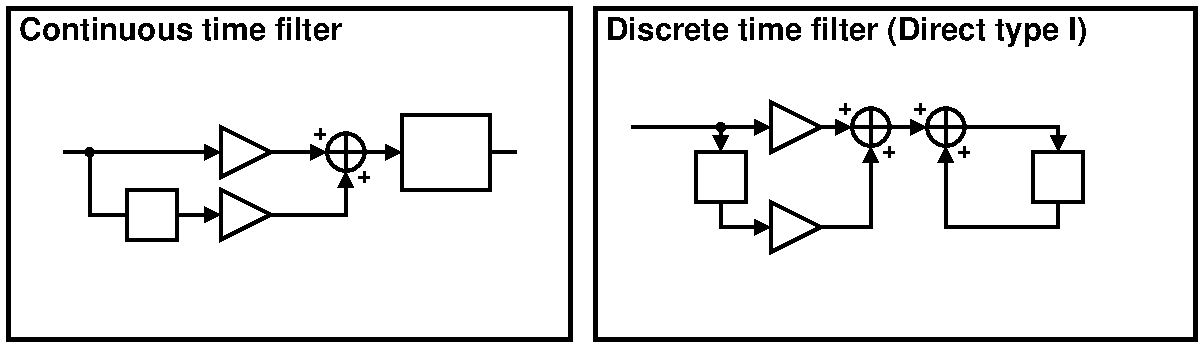
\includegraphics[scale=0.70000]{./figs/filter_arch_pi.pdf}\\
   % translate x=1728 y=944 scale 0.38
   \putbox{1.91800in}{0.90300in}{0.96}{$\frac{1}{\frac{s}{\omega_p} + 1}$}%
   \putbox{1.14800in}{1.01500in}{0.96}{$K_p$}%
   \putbox{1.14800in}{0.72800in}{0.96}{$K_i$}%
   \putbox{0.60900in}{0.58100in}{0.96}{$1/s$}%
   \putbox{0.25900in}{0.98700in}{0.96}{x[n]}%
   \putbox{2.35900in}{0.98700in}{0.96}{y[n]}%
   \putbox{2.92600in}{1.10600in}{0.96}{x[n]}%
   \putbox{4.99800in}{1.01500in}{0.96}{\rotatebox{-360}{y[n]}}%
   \putbox{3.26200in}{0.75600in}{0.96}{$z^{-1}$}%
   \putbox{3.73100in}{1.13400in}{0.96}{b$_0$}%
   \putbox{3.73100in}{0.66500in}{0.96}{b$_1$}%
   \putbox{4.83700in}{0.75600in}{0.96}{$z^{-1}$}%
   \putbox{4.99800in}{0.55300in}{0.96}{y[n-1]}%
   } % close 'parbox'
   } % close 'scalebox'
   \vspace{-\baselineskip} % this is not necessary, but looks better
\fontfamily{\rmdefault}\selectfont
